% From reconfigurable architectures to self-adaptive autonomic systems 
\cite{reconfigurable} proposes the harvesting of the full potential of dynamic reconfiguration by carefulyl evaluating the overhead of reconfiguration in hardware-software interfacing. To overcome the limits introduced by increasing complexity and the workloads to maintain complex infrastructues they propose to adopt a codesigned self-adaptive and autonomic computing system. 
%A full \emph{bitstream} configures the whole configuration memory statically at the beginning of the execution of a system, while partial bitstreams are used for reconfiguration to confirgure merely portions of the device. 

\emph{Partial dynamic reconfiguration (PRD)} is a key feature that makes FPGAs unique. PDR addresses the lack of resources to implement an application and its adaptability needs. Reconfigurable hardware taking advantage of partial dynamic reconfiguration is the perfect trade-off between the speed of HW and the flexibility of SW. \cite{reconfigurable} presents an evaluation system, implemented on the Xilinx Virtex-II Pro VP30 on an architecture of two reconfigurable cores. Running an extended version of Linux, the cores can be partial dynamically reconfigured. They compare the performance of three different impementations of a popular encryption algorithm (advanced encryption standard): a reconfigurable IP-core that is configured at runtime (FPGA-RHW), a cached hardware IP-core that is ready to use (FPGA-CHW) and a software implementation (SW). 
% -- reconfig, cached & software ---------------------------
\begin{figure}[htb]%
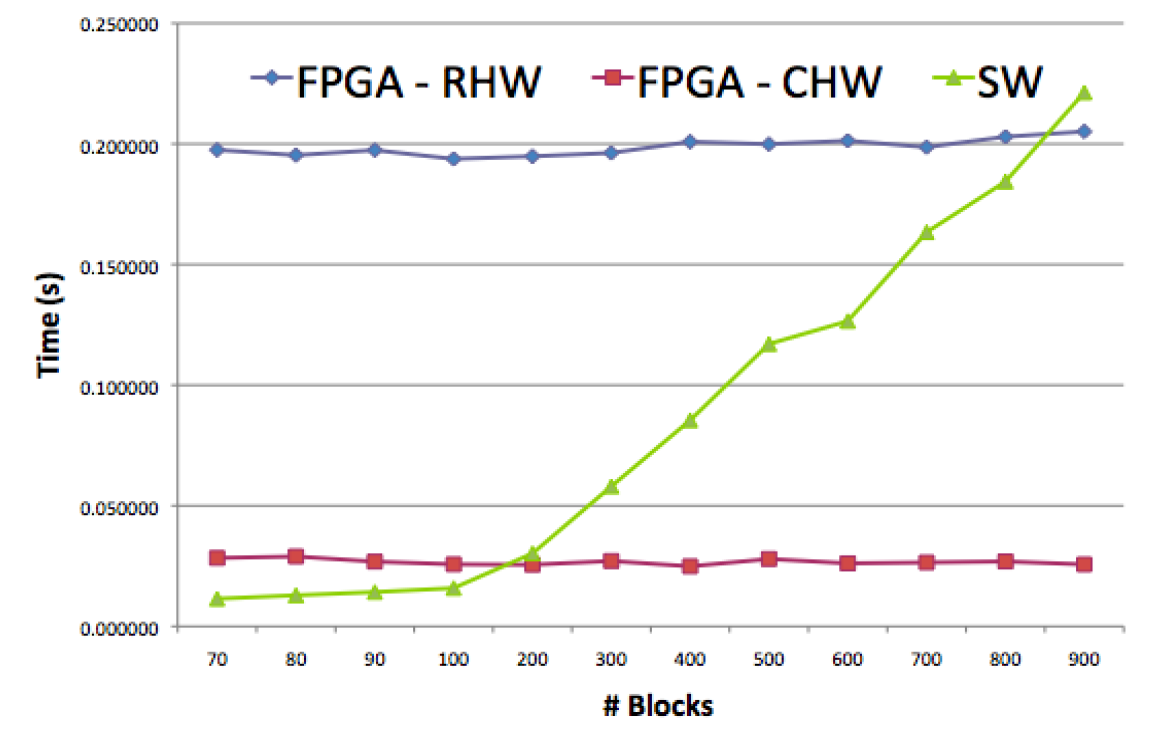
\includegraphics[width=\columnwidth]{Pictures/reconfig.png}%
\caption{Execution time of the implementations of the AES algorithm as seen in \cite{reconfigurable}}%
\label{fig:reconfig}%
\end{figure} 
Figure \ref{fig:reconfig} displays the overhead introduced by reconfiguration when comparing the three implementations. Even though this data was captured in a static analysis, it displays that reconfiguration may dominate the execution in smaller systems as reconfiguration seems to be only valid in systems of larger than 900 processed blocks. This shows the need for an efficient and fast decision engine and switching protocol. 
%
%However, an important problem often neglected is the time overhead the reconfiguration process introduces and the two-dimensional partitioning strategy reconfigurable devices need: spatial and temporal. \cite{reconfigurable} presents the urge to carefully evaluate the overhead created as a negative impact of reconfiguration latency which is not always discussed in present papers. 